% -*- root: ../main.tex -*-
\chapter{Design di Dettaglio}
In questo capitolo verrà spiegato come si è giunti a realizzare l’applicativo,
confrontando poi i mockup con le effettive interfacce utente, descrivendone i componenti e infine mostrando lo schema della base di dati implementata.

Come tutti i programmi, il progetto è costituito da  frontend e backend.
Questi denotano rispettivamente la parte visibile all'utente di un programma e con cui egli può interagire —tipicamente un'interfaccia utente— e la parte che permette l'effettivo funzionamento di queste interazioni. \newline
Il frontend, nella sua accezione più generale, è responsabile dell'acquisizione dei dati di ingresso e della loro elaborazione con modalità conformi a specifiche predefinite e invarianti, tali da renderli utilizzabili dal backend. Il collegamento del frontend al backend è un caso particolare di interfaccia.

\section{Frontend}
Fin dall'analisi del progetto è stato chiaro che il target dell'applicazione fosse ampio, infatti l'insieme degli utenti interessati comprende chiunque abbia la
necessità di consultare delle previsioni meteo.
Per questo motivo, le interfacce e il funzionamento dell'applicazione sono stati progettati per essere adoperati anche dagli utenti meno esperti.

\subsection{Interfacce utente}
In seguito ad un'analisi preliminare del problema sono stati prodotti dei mockup della grafica per dare l'idea delle funzioni e dei requisiti dell'applicativo. 
Le pagine effettive si sono evolute durante lo sviluppo ma mantengono le linee guida dei mockup. 
Vengono descritte le interfacce utente più importanti.
Si consulti anche il capitolo \ref{prodottofinale} per visualizzare il risultato finale delle pagine.

\begin{figure}[H]
    \caption{Home}
    \label{fig:Home}
    \centering
    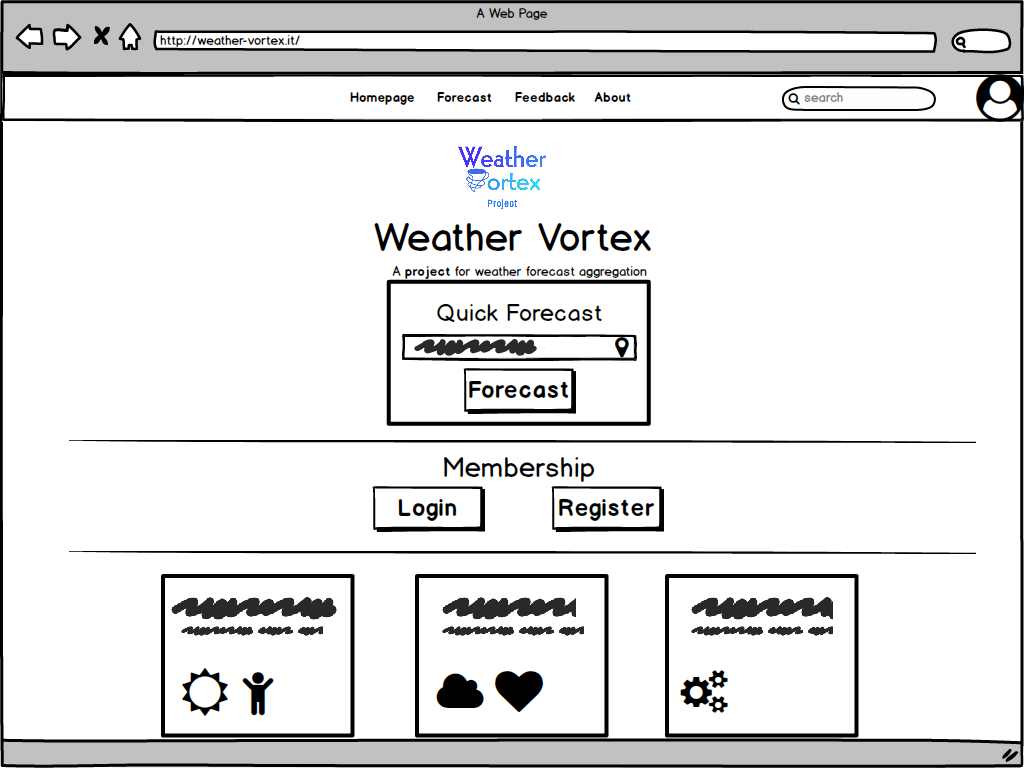
\includegraphics[width=0.6\textwidth]{MockUps/homepage.png}
\end{figure}
La homepage è la pagina principale di presentazione.
In bella vista presenta una card con una barra di testo dove inserire il nome della località con l'icona di una mappa per le coordinate geografiche, con due bottoni in basso per richiedere le previsioni. 
Attraverso i bottoni Login e Register inoltre si può accedere alle pagine di autenticazione.

\begin{figure}[H]
    \caption{Login}
    \label{fig:Login}
    \centering
    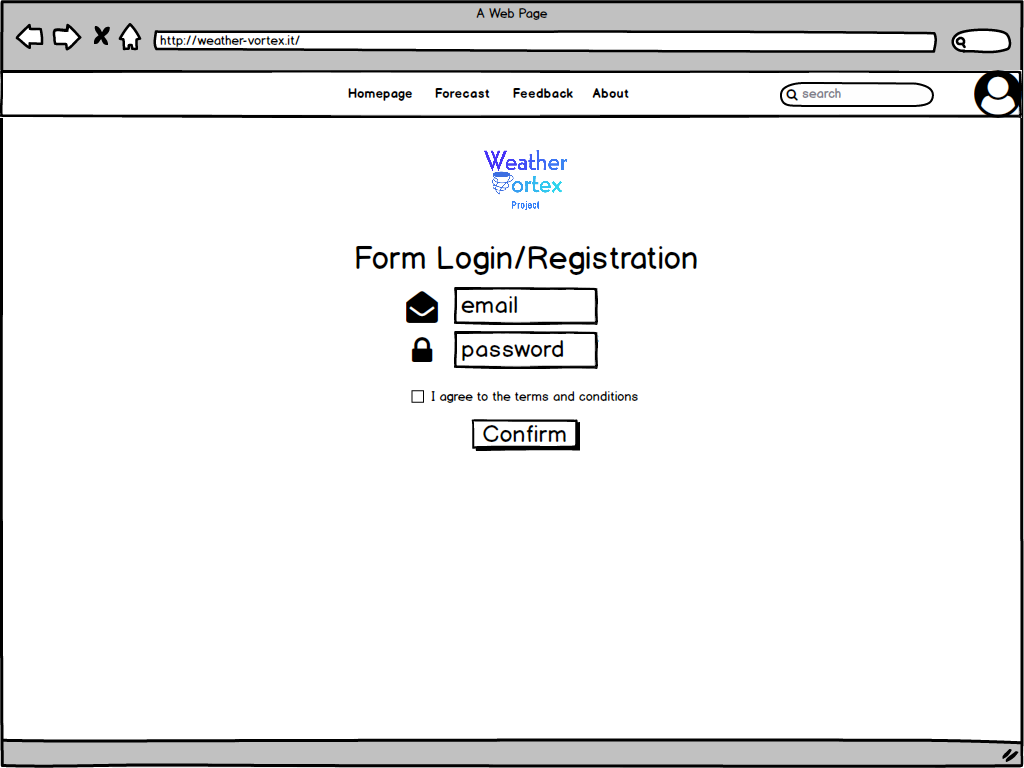
\includegraphics[width=0.6\textwidth]{MockUps/Login_Register.png}
\end{figure}
Viene pensata una pagina di login classica con la possibilità di recuperare la password e una pagina di registrazione. Effettuata la registrazione viene chiesto agli utenti di completare la propria iscrizione cliccando sul link dell'email di conferma.

\begin{figure}[H]
    \caption{Forecast}
    \label{fig:Forecast}
    \centering
    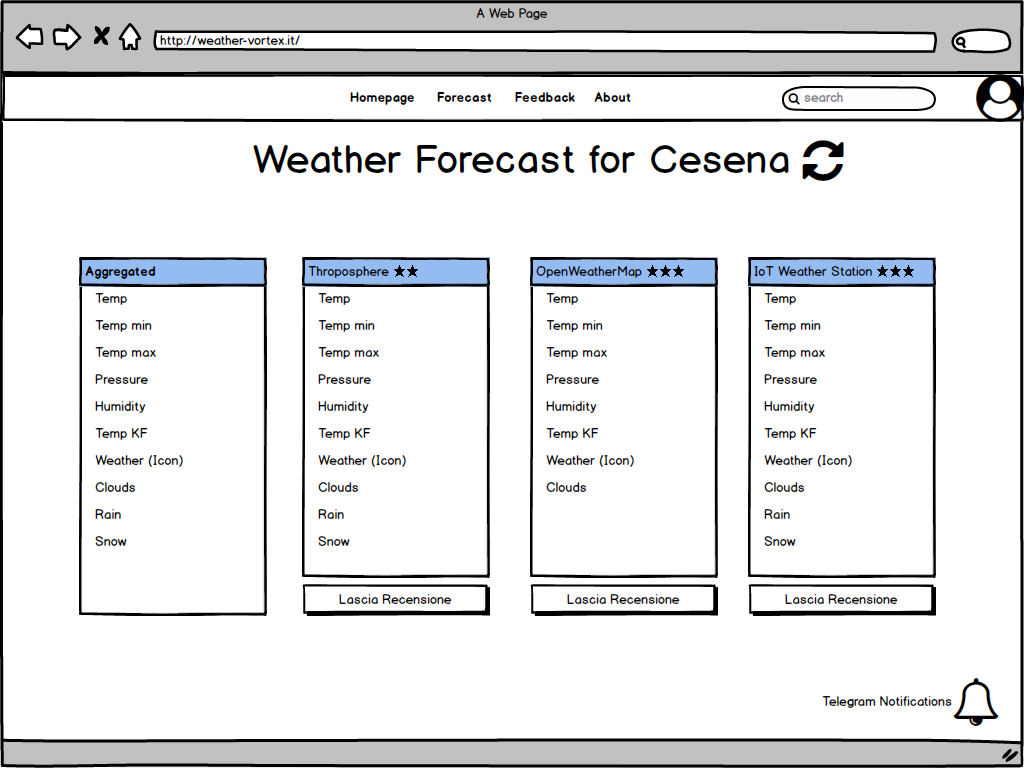
\includegraphics[width=0.6\textwidth]{MockUps/forecast.png}
\end{figure}
Il fulcro dell'applicazione è sicuramente la pagina delle previsioni. Inizialmente la pagina visualizza un'immagine esplicativa con in alto una barra di testo dove inserire la località oppure richiedere le coordinate geografiche attuali attraverso l'icona della mappa. Cliccando sui due pulsanti a lato si può richiedere il meteo attuale o quello dei prossimi tre giorni. Comparirà così in posizione centrale la card della previsione aggregata e in basso un insieme di schede che rappresentano le previsioni di ogni provider, con informazioni utili sul meteo.
 Nel caso siano richieste le previsioni dei prossimi tre giorni, la pagina si aggiornerà mettendo a disposizione un tooltip di bottoni per scegliere il giorno specifico e uno slider per scegliere l'ora della previsione.

\begin{figure}[H]
    \caption{Feedbacks}
    \label{fig:Feedbacks}
    \centering
    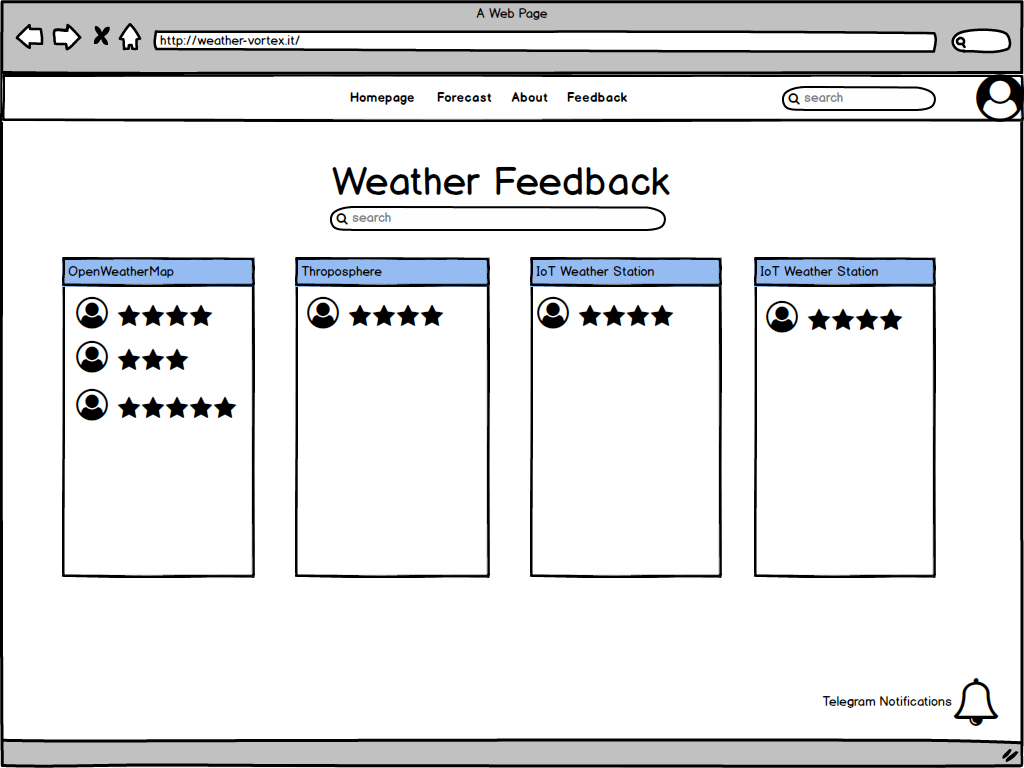
\includegraphics[width=0.6\textwidth]{MockUps/feedback.png}
\end{figure}
Nella pagina delle recensioni è possibile visualizzare uno slider che contiene le schede con le recensioni relative ai vari provider. Tramite la barra di ricerca in alto è possibile trovare quello desiderato digitandone parte del nome. Ogni scheda contiene una lista di recensioni lasciate dagli utenti. Per ogni recensione viene mostrato l'avatar dell'utente che l'ha rilasciata, con a lato la sua valutazione. Questa è stata espressa graficamente da una a cinque stelle. Cliccando sul campo è possibile visualizzare il profilo pubblico dell'utente associato.

\begin{figure}[H]
    \caption{Aggiunta di una recensione}
    \label{fig:FeedbacksDialog}
    \centering
    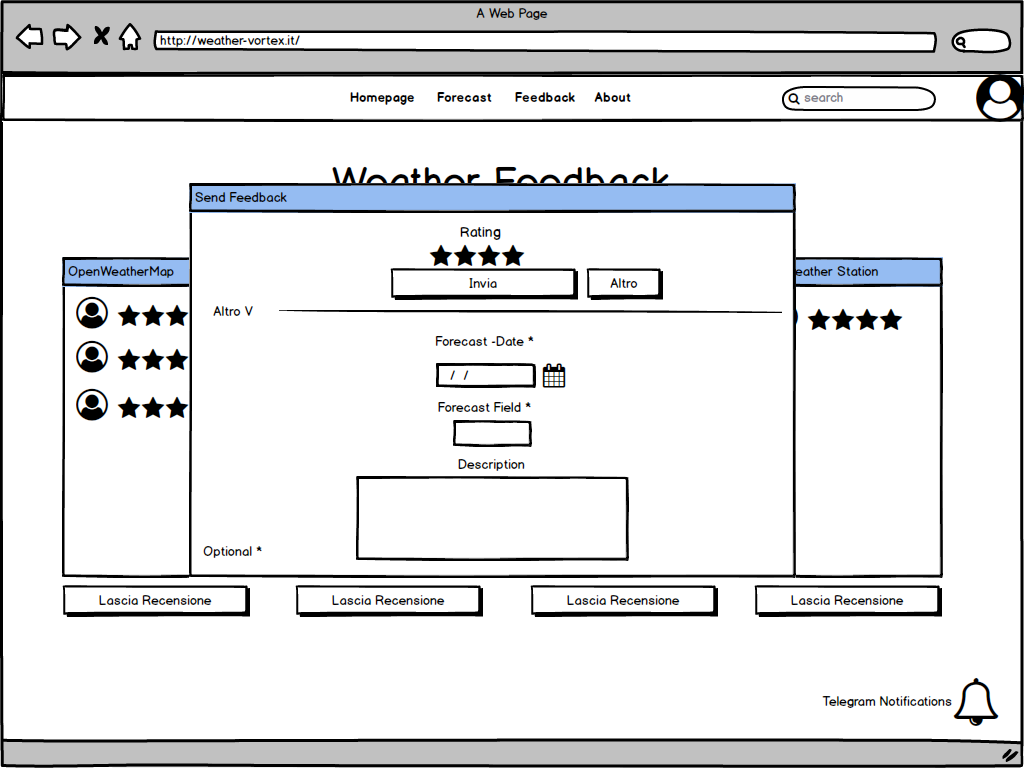
\includegraphics[width=0.6\textwidth]{MockUps/sendFeedback.png}
\end{figure}

All'estremità di ogni scheda, se si è autenticati, sarà presente il pulsante per aggiungere una nuova recensione. Se si clicca su di esso si visualizzerà una finestra con il rating da inserire. Questa è espandibile: si possono anche specificare il campo della previsione che si vuole recensire (ad esempio temperatura minima, Pressione, etc), la data della previsione alla quale ci si riferisce, e eventuali note.
In cima ad ogni card si è deciso di far visualizzare una statistica, calcolata come media dei rating di quel provider. Si tratta di un indice di affidabilità che calcola l'accuratezza della previsione, basandosi sull'opinione delle altre persone.

\begin{figure}[H]
    \caption{Private Profile}
    \label{fig:PrivateProfile}
    \centering
    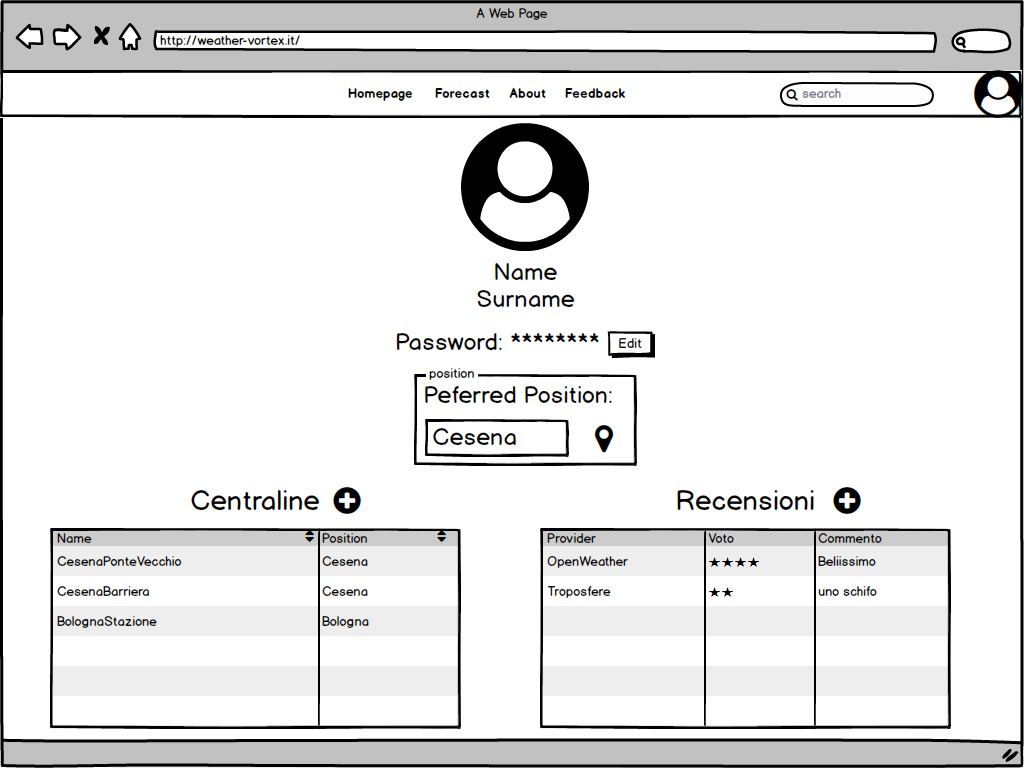
\includegraphics[width=0.6\textwidth]{MockUps/Private Profile.png}
\end{figure}
La pagina del profilo privato dà la possibilità ad ogni utente di visualizzare e gestire le proprie informazioni personali. Cliccando su "edit" si aprirà un dialog che consentirà di poter modificare la propria password o la propria posizione preferita.
L'utente ha la possibilità di visualizzare le proprie centraline, di aggiungerle tramite il pulsante "+" in alto della tabella, modificarle e eventualmente cancellarle (ne verrà richiesta la conferma).
L'utente ha la possibilità di visualizzare le proprie recensioni e eventualmente cancellarle (ne verrà richiesta la conferma).
Navigando in questa pagina c'è anche la possibilità di cancellare il proprio account tramite un bottone apposito in fondo alla pagina.

La pagina del Profilo pubblico ha la stessa struttura del Profilo privato, ma qui nessuna operazione di modifica è concessa.

\begin{figure}[H]
    \caption{About}
    \label{fig:About}
    \centering
    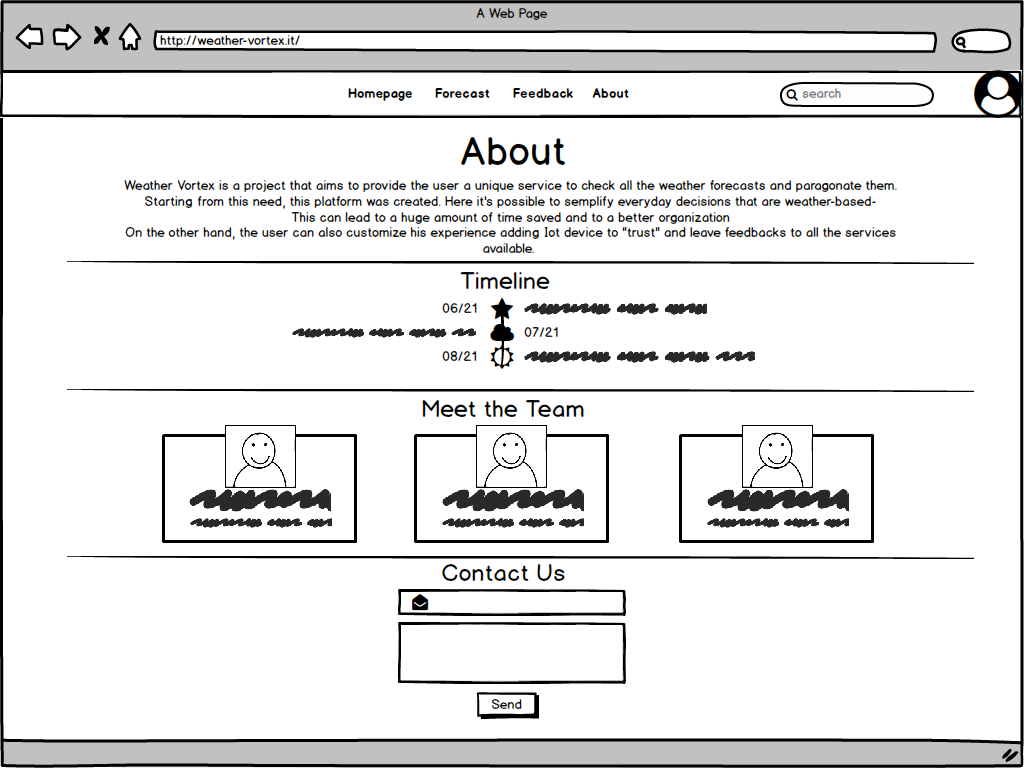
\includegraphics[width=0.6\textwidth]{MockUps/about.png}
\end{figure}
Infine una pagina per i contatti che consente l'inserimento di un messaggio/ticket
per il supporto tecnico e alcune informazioni sul team di sviluppo.

\subsection{Componenti}
Si descrivono in breve i componenti principali usati per ogni pagina.
Prima di tutto si elencano i componenti presenti in tutte le pagine:
\begin{itemize}
    \item Appbar:  E' una barra colorata situata nella zona alta della pagina. Contiene tre componenti:
    \begin{itemize}
    \item Icona Utente: Situata nell'estremità destra, permette di autenticarsi o registrarsi al sito se l'utente non ha eseguito l'accesso, altrimenti esso può visualizzare la propria pagina del profilo privato o effettuare il logout. Il suo aspetto cambia: se è autenticato mostra le iniziali del proprio nome e cognome, altrimenti mostra un'icona generica. 
    \item Titolo Weather Vortex: Situata nella parte centrale, permette di navigare alla home cliccando su di esso.
    \item Icona Menù: Situata nell'estremità sinistra, consente di mostrare o nascondere la barra di navigazione (Navbar).
    \end{itemize}
    \item Navbar: Si tratta della barra di navigazione attraverso cui l'utente può muoversi nelle principali finestre del sito.
    \item Footer: Il footer a fine pagina contenente dei link utili.
\end{itemize}
La pagina Home è composta dai principali componenti:
\begin{itemize}
    \item QuickForecastCard: Card che viene usata come scorciatoia per visualizzare le previsioni. 
    \item AccountButtons: Contiene i bottoni per accedere alle pagine di autenticazione.
    \item InfoMain: Insieme di cards di descrizione
    \item checkStatus: Card che mostra lo stato del server.
\end{itemize}
La pagina Feedbacks è composta dai seguenti componenti:
\begin{itemize}
    \item SlidesOrizontalGroup: Si tratta dello slider che contiene le schede dei vari provider con le recensioni. E' composto da due sottocomponenti:
    \begin{itemize}
        \item ServiceRatingList: Rappresenta la lista delle recensioni del provider. Ogni campo recensione è composto dall'avatar dell'utente, dalle sue iniziali e dalla sua recensione.
        \item FeedbackDialog: Rappresenta il dialog per l'aggiunta della recensione.
    \end{itemize}
\end{itemize}
La pagina Forecast è composta dai seguenti componenti:
\begin{itemize}
    \item EmptyForecast: Mostra la pagina iniziale delle previsioni.
    \item CurrentForecast: Mostra la pagina del meteo attuale. E' composta dal seguente sottocomponente: 
    \begin{itemize}
    \item ForecastGroup. Esso rappresenta l'insieme delle previsioni meteo. Richiama il componente WeatherForecastCard che rappresenta una singola previsione per uno specifico provider o il meteo aggregato. Esso contiene la descrizione del meteo, la data, la temperatura minima e massima, la pressione, l'umidità, la quantità di nuvole, di pioggia e di neve. 
    \end{itemize}
    \item ThreeDaysForecast: Mostra la pagina delle previsioni dei prossimi tre giorni. Richiama gli stessi componenti di "CurrentForecast".
\end{itemize}
La pagina Profilo Privato è composta dai seguenti componenti:
\begin{itemize}
    \item PrivateUserCard: Si tratta della card che visualizza le informazioni private dell'utente: avatar, nome, cognome, data di creazione, email, posizione preferita e bottone di modifica.
    \item PrivateUserReviews: Tabella che visualizza le recensioni rilasciate. Contiene i relativi campi: provider, valutazione, commento e un pulsante per la cancellazione.
    \item PrivateUserControlUnits: Tabella che visualizza tutte le centraline inserite. E' costituita dai seguenti campi: nome, posizione, url e due pulsanti per la modifica e la cancellazione.

\end{itemize}
La pagina Profilo Pubblico ha i seguenti sottocomponenti:
\begin{itemize}
    \item PublicUserCard: Si tratta della card che visualizza le informazioni pubbliche dell'utente: avatar, nome, cognome, eventuale posizione preferita.
    \item PublicUserReviews: Tabella che mostra le recensioni lasciate dall'utente. Contiene i seguenti campi: provider, recensione, commento.
    \item PublicUserControlUnits: Tabella che visualizza tutte le centraline inserite dell'utente. E' costituita dai seguenti campi: nome, posizione, url.

\end{itemize}   
La pagina About è composta dai seguenti componenti:
\begin{itemize}
    \item Timeline: Componente che visualizza cronologicamente gli vari stadi del progetto.
    \item MeetTeam: Un insieme di cards per descrivere gli autori del progetto. 
    \item ContactUs: Componente che funge da modulo di contatto.
\end{itemize}
\subsection{Vue-Router}
Oltre ai componenti descritti sopra all'interno di ogni pagina un componente di Vue.js che è stato utilizzato è il vue-router, per il routing e la navigazione delle pagine.
Esso consente, tramite una router-view, di visualizzare i componenti
desiderati (che insieme compongono le varie interfacce utente).
\section{Backend}
Viene ora mostrato lo schema di database utilizzato dall'applicazione:
\begin{figure}[H]
    \caption{Database}
    \label{fig:Database}
    \centering
    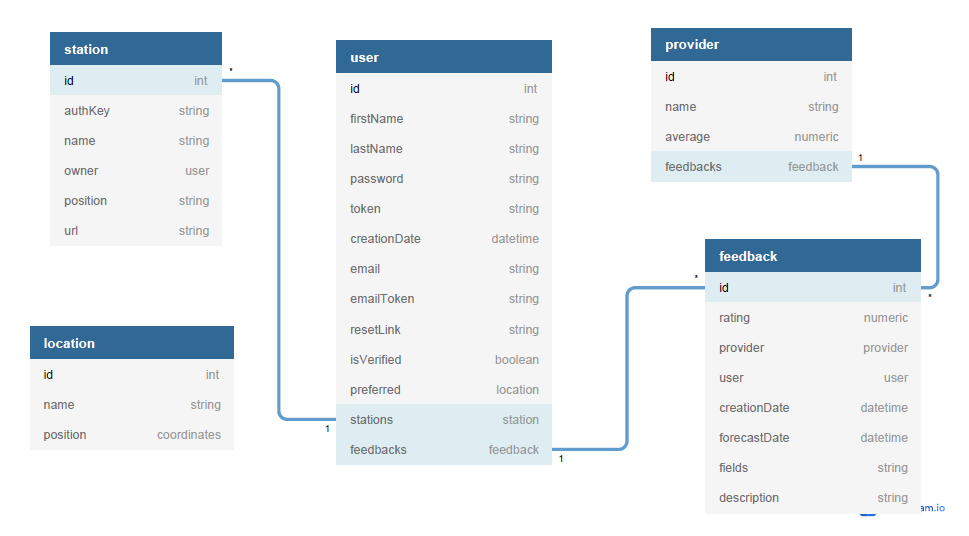
\includegraphics[width=1.0\textwidth]{DrawIo/database.png}
\end{figure}
\subsection{Modelli}
Ci sono cinque modelli
che sono il fulcro dell'applicazione, essi si trovano nella cartella models. Essi costituiscono un modello di dati da salvare in MongoDB, che vengono usati per istanziare oggetti che saranno automaticamente dotati di metodi per svolgere le classiche operazioni CRUD.
\begin{itemize}
\item user - Rappresenta il modello dell'utente. I suoi campi sono:
\begin{itemize}
\item firstName: nome dell'iscritto.
\item lastName: cognome dell'iscritto.
\item password: password dell'iscritto.
\item email: email dell'iscritto.
\item token: stringa generata durante il login per verificare l'autenticazione dell'utente.
\item creationDate: data di creazione dell'account.
\item emailToken: token per verificare l'iscrizione.
\item resetLink: token per il cambio della password.
\item isVerified: booleano che indica se l'utente è stato verificato.
\item preferred: una eventuale località preferita.
\item stations: elenco delle centraline dell'utente.
\item feedbacks: elenco delle recensioni dell'utente.
\end{itemize}
\item feedback - Rappresenta il modello della recensione. I suoi campi sono: 
\begin{itemize}
    \item rating: valutazione della recensione. 
    \item provider: il provider a cui la recensione si riferisce.
    \item user: utente che ha rilasciato la recensione.
    \item creationData: data di creazione della recensione.
    \item forecastData: data della previsione su cui si è basata la valutazione della recensione.
    \item fields: eventuali campi della previsione da valutare.
    \item description: eventuale descrizione.
\end{itemize}
\item location - Rappresenta il modello della località. I suoi campi sono:
\begin{itemize}
    \item name: nome della località.
    \item position: posizione della località espressa in coordinate geografiche tramite latitudine e longitudine.
\end{itemize}
Serve per memorizzare le richieste di previsioni che sono state fatte.
\item provider - Rappresenta il modello del provider che fornisce il meteo. I suoi campi sono:
\begin{itemize}
    \item name: nome del provider.
    \item average: la media di tutte le valutazioni date al provider.
    \item feedbacks: lista di tutte le recensioni del provider date dagli utenti.
\end{itemize}
\item station - Rappresenta  il modello della centralina. I suoi campi sono:
\begin{itemize}
    \item authKey: valore usato per autenticare richieste alla stazione.
    \item name: nome della centralina.
    \item owner: proprietario della centralina.
    \item position: nome della località in cui si trova.
    \item url: url della centralina.
\end{itemize}
\end{itemize}
\subsection{Storage}
Gli storage sono dei componenti che si occupano di manipolare i dati e i modelli dell'applicazione nascondendo il supporto di memorizzazione degli stessi. 
\begin{itemize}
\item{database storage} - storage che usa come supporto di memorizzazione il database.
\item{webservice storage} - storage che richiede i dati ad un web service esterno. Nella nostro caso si tratta di gestire le richieste da provider esterni e recuperarne le previsioni.


\end{itemize}





